\documentclass[a4paper,14pt,oneside,final]{extarticle}
\usepackage[top=2cm, bottom=2cm, left=3cm, right=1cm]{geometry}
\usepackage{scrextend}

\usepackage[T2A,T1]{fontenc}
\usepackage[ukrainian,russian,english]{babel}
\usepackage{tempora}
\usepackage{fontspec}
\setmainfont{tempora}

% Зачем: Отключает использование изменяемых межсловных пробелов.
% Почему: Так не принято делать в текстах на русском языке.
\frenchspacing

\usepackage{indentfirst}
\setlength{\parindent}{1.25cm}
\renewcommand{\baselinestretch}{1.5}

% Header
\usepackage{fancyhdr}
\pagestyle{fancy}
\fancyhead{}
\fancyfoot{}
\fancyhead[R]{\small \selectfont \thepage}
\renewcommand{\headrulewidth}{0pt}

% Captions
\usepackage{chngcntr}
\counterwithin{figure}{section}
\counterwithin{table}{section}
\usepackage[tableposition=top]{caption}
\usepackage{subcaption}
\DeclareCaptionLabelFormat{gostfigure}{Рисунок #2}
\DeclareCaptionLabelFormat{gosttable}{Таблиця #2}
\DeclareCaptionLabelSeparator{gost}{~---~}
\captionsetup{labelsep=gost}
\captionsetup[figure]{labelformat=gostfigure}
\captionsetup[table]{labelformat=gosttable}
\renewcommand{\thesubfigure}{\asbuk{subfigure}}

% Sections
\usepackage[explicit]{titlesec}
\newcommand{\sectionbreak}{\clearpage}

\titleformat{\section}
  {\centering}{\thesection \quad}{0pt}{\MakeUppercase{#1}}
\titleformat{\subsection}[block]
  {\bfseries}{\thesubsection \quad #1}{0cm}{}

\titlespacing{\section} {0cm}{0cm}{21pt}
\titlespacing{\subsection} {\parindent}{21pt}{0cm}
\titlespacing{\subsubsection} {\parindent}{0cm}{0cm}

% Lists
\usepackage{enumitem}
\renewcommand\labelitemi{--}
\setlist[itemize]{noitemsep, topsep=0pt, wide}
\setlist[enumerate]{noitemsep, topsep=0pt, wide, label=\arabic*}
\setlist[description]{labelsep=0pt, noitemsep, topsep=0pt, leftmargin=2\parindent, labelindent=\parindent, labelwidth=\parindent, font=\normalfont}

% Toc
\usepackage{tocloft}
\tocloftpagestyle{fancy}
\renewcommand{\cfttoctitlefont}{}
\setlength{\cftbeforesecskip}{0pt}
\renewcommand{\cftsecfont}{}
\renewcommand{\cftsecpagefont}{}
\renewcommand{\cftsecleader}{\cftdotfill{\cftdotsep}}

\usepackage{float}
\usepackage{pgfplots}
\usepackage{graphicx}
\usepackage{multirow}
\usepackage{amssymb,amsfonts,amsmath,amsthm}
\usepackage{csquotes}

\usepackage{listings}
\lstset{basicstyle=\footnotesize\ttfamily,breaklines=true}
\lstset{language=Matlab}

\usepackage[
	backend=biber,
	sorting=none,
	language=auto,
	autolang=other
]{biblatex}
\DeclareFieldFormat{labelnumberwidth}{#1}

\lstdefinelanguage{Python}{
  keywords={and, break, class, continue, def, yield, del, elif, else, except, exec, finally, for, from, global, if, import, in, lambda, not, or, pass, print, raise, return, try, while, assert, with},
  keywordstyle=\color{NavyBlue}\bfseries,
  ndkeywords={True, False},
  ndkeywordstyle=\color{BurntOrange}\bfseries,
  emph={as},
  emphstyle={\color{OrangeRed}},
  identifierstyle=\color{black},
  sensitive=true,
  commentstyle=\color{gray}\ttfamily,
  comment=[l]{\#},
  morecomment=[s]{/*}{*/},
  stringstyle=\color{ForestGreen}\ttfamily,
  morestring=[b]',
  morestring=[s]{"""*}{*"""},
}


\newcommand{\labnumber}{5} % fifth lab
\documentclass[a4paper,14pt,oneside,final]{extarticle}
\usepackage[top=2cm, bottom=2cm, left=3cm, right=1cm]{geometry}
\usepackage{scrextend}

\usepackage[T2A,T1]{fontenc}
\usepackage[ukrainian,russian,english]{babel}
\usepackage{tempora}
\usepackage{fontspec}
\setmainfont{tempora}

% Зачем: Отключает использование изменяемых межсловных пробелов.
% Почему: Так не принято делать в текстах на русском языке.
\frenchspacing

\usepackage{indentfirst}
\setlength{\parindent}{1.25cm}
\renewcommand{\baselinestretch}{1.5}

% Header
\usepackage{fancyhdr}
\pagestyle{fancy}
\fancyhead{}
\fancyfoot{}
\fancyhead[R]{\small \selectfont \thepage}
\renewcommand{\headrulewidth}{0pt}

% Captions
\usepackage{chngcntr}
\counterwithin{figure}{section}
\counterwithin{table}{section}
\usepackage[tableposition=top]{caption}
\usepackage{subcaption}
\DeclareCaptionLabelFormat{gostfigure}{Рисунок #2}
\DeclareCaptionLabelFormat{gosttable}{Таблиця #2}
\DeclareCaptionLabelSeparator{gost}{~---~}
\captionsetup{labelsep=gost}
\captionsetup[figure]{labelformat=gostfigure}
\captionsetup[table]{labelformat=gosttable}
\renewcommand{\thesubfigure}{\asbuk{subfigure}}

% Sections
\usepackage[explicit]{titlesec}
\newcommand{\sectionbreak}{\clearpage}

\titleformat{\section}
  {\centering}{\thesection \quad}{0pt}{\MakeUppercase{#1}}
\titleformat{\subsection}[block]
  {\bfseries}{\thesubsection \quad #1}{0cm}{}

\titlespacing{\section} {0cm}{0cm}{21pt}
\titlespacing{\subsection} {\parindent}{21pt}{0cm}
\titlespacing{\subsubsection} {\parindent}{0cm}{0cm}

% Lists
\usepackage{enumitem}
\renewcommand\labelitemi{--}
\setlist[itemize]{noitemsep, topsep=0pt, wide}
\setlist[enumerate]{noitemsep, topsep=0pt, wide, label=\arabic*}
\setlist[description]{labelsep=0pt, noitemsep, topsep=0pt, leftmargin=2\parindent, labelindent=\parindent, labelwidth=\parindent, font=\normalfont}

% Toc
\usepackage{tocloft}
\tocloftpagestyle{fancy}
\renewcommand{\cfttoctitlefont}{}
\setlength{\cftbeforesecskip}{0pt}
\renewcommand{\cftsecfont}{}
\renewcommand{\cftsecpagefont}{}
\renewcommand{\cftsecleader}{\cftdotfill{\cftdotsep}}

\newcommand{\khpistudentgroup}{КН-34г}
\newcommand{\khpistudentname}{Чепурний~А.~С.}

\newcommand{\khpidepartment}{Програмна інженерія та інформаційні технології управління}
\newcommand{\khpititlewhat}{
	Лабораторна робота №\labnumber \\
	з предмету <<Моделювання систем>>
}
\newcommand{\khpititlewho}{
	Виконав: \\
	\hspace*{\parindent} ст. групи \khpistudentgroup \\
	\hspace*{\parindent} \khpistudentname \\
	Перевірила: \\
	\hspace*{\parindent} ст. в. каф. ПІІТУ \\
	\hspace*{\parindent} Єршова~С.~І. \\
	\hspace*{\parindent} ас. каф. ПІІТУ \\
	\hspace*{\parindent} Литвинова~Ю.~С. \\
}



\usepackage{longtable,tabu}

\graphicspath{{figures/}}

\begin{document}
\Ukrainian

\begin{titlepage}

\begin{center}
	МІНІСТЕРСТВО ОСВІТИ І НАУКИ УКРАЇНИ \\
	НАЦІОНАЛЬНИЙ ТЕХНІЧНИЙ УНІВЕРСИТЕТ \\
	«ХАРКІВСЬКИЙ ПОЛІТЕХНІЧНИЙ ІНСТИТУТ» \\[0.5cm]
	Кафедра <<\khpidepartment>> \\
\end{center}

\vspace{6cm}

\begin{center}
	\khpititlewhat
\end{center}

\vspace{3cm}

\begin{addmargin}[10cm]{0cm}
	\khpititlewho
\end{addmargin}

\vspace{\fill}

\begin{center}
	Харків \the\year
\end{center}

\end{titlepage}

\addtocounter{page}{1}

\section{Cервер и инструментальные средства MongoDB}
\subsection*{Цель}
Анализ кластера MongoDB
\subsection*{Задачи}
\begin{itemize}
	\item проанализировать возможности, предоставляемые MongoDB;
	\item проанализировать этапы развертывания кластера MongoDB;
	\item проанализировать структуру кластера MongoDB.
\end{itemize}

\subsection{Возможности MongoDB}
Для решения проблем настройки, машстабування и синхронизации кластера MongoDB предоставляет два основных механизма, такие как репликация и шардинг.

Репликация --- это процесс синхронизации данных между несколькими серверами. Репликация обеспечивает избыточность и повышает доступность данных благодаря наличию нескольких копий данных на различных серверах баз данных. Репликация защищает базу данных от потери одного сервера. Репликация также позволяет восстанавливаться после сбоя оборудования и перерывов в обслуживании. С дополнительными копиями данных можно выделить одну для аварийного восстановления, создания отчетов или резервного копирования.

Предоставляющая репликация:
\begin{itemize}
	\item высокая доступность данных;
	\item аварийное восстановление;
	\item масштабирование чтения (дополнительные копии для чтения)
	\item набор реплик прозрачен для приложения.
\end{itemize}

MongoDB достигает репликации с помощью набора реплик. Набор реплик - это группа экземпляров mongod, содержащие один и тот же набор данных. В реплике один узел является основным узлом, который получает все операции записи. Все остальные экземпляры, такие как вторичные, применяют операции по первичному, чтобы у них был тот же набор данных. Набор реплик может иметь только один основной узел.

Набор реплик --- это группа из двух или более узлов (обычно требуется минимум 3 узла).

В наборе реплик один узел является первичным узлом, а другие узлы являются вторичными. Все данные реплицируются с первичного на вторичный узел.
Во время автоматического восстановления после сбоя или обслуживания выбор устанавливается для основного и новый основной узел выбирается. После восстановления отказал узла он снова присоединяется к набору реплик и работает как вторичный узел.

Шардинг (Sharding) --- это процесс хранения записей данных на нескольких машинах, и этот подход MongoDB к удовлетворению требований роста данных. Поскольку размер данных увеличивается, одной машины может быть недостаточно для хранения данных или обеспечения приемлемой скорости чтения и записи. Шардинг решает проблему с горизонтальным масштабированием. С помощью шардинга возможно добавить больше машин для поддержания роста данных и требований операций чтения и записи.

Преимущества шардинга:
\begin{itemize}
	\item при репликации все записи идут на главный узел;
	\item запросы, чувствительные к задержке прежнему отправляются мастеру;
	\item один набор реплик имеет ограничения в 12 узлов;
	\item память не может быть достаточно большой, когда активный набор данных большой;
	\item локальный диск недостаточно большой;
	\item вертикальное масштабирование слишком дорогое.
\end{itemize}

\subsection{Этапы развертывания кластера MongoDB}
Развертывание кластера возможно без использования механизмов масштабирования. Такой способ используется для разработки, достаточно мало нагруженных сервисов. Зачастую используют только механизм репликации, так как он предоставляет такую ​​основную преимущества как доступность и восстановления данных. Шардинг используют только в том случае, если вертикальное масштабирование будет стоить больше чем горизонтальное. Так как для шардинга необходимо еще оптимально настроить правила для распределения данных на шарды.

Для примера рассмотрим развертывание кластера с использованием механизма шардинга, так как это позволит MongoDB обрабатывать большие объемы данных.
Разворачивать будем локально на linux ubuntu 18.04. Для развертывания нам понадобится установленная ​​MongoDB.

Последовательность действий:

Создадим 2 пустые директории, в которых будут храниться данные:
\begin{lstlisting}
> sudo mkdir /data/instance1
> sudo mkdir /data/instance2
\end{lstlisting}

Поднимаем 2 инстанса mongodb командами:
\begin{lstlisting}
> sudo mongod --dbpath /data/instance1 --port 27000
> sudo mongod --dbpath /data/instance2 --port 27001
\end{lstlisting}

Создадим пустую директорию, в которой будут храниться данные конфигурации сервера:
\begin{lstlisting}
> sudo mkdir /data/config
\end{lstlisting}

Поднимаем конфиг сервер командой
\begin{lstlisting}
> sudo mongod --configsvr --dbpath /data/config --port 27002
\end{lstlisting}

Параметр \texttt{--configsvr} указывает, что новый инстанс будет именно конфиг сервером, --dbpath --- путь, по которому будут храниться данные.

Запускаем mongos командой:
\begin{lstlisting}
> sudo mongos --configdb 127.0.0.1:27002 --port 27100
\end{lstlisting}

По этой команде поднимается mongos на порту 27100, на вход ему нужно передать перечень конфиг серверов с их хостами, на которые он будет обращаться. Если мы при поднятии монгоса не указали порт, то он использует по умолчанию 27017

Необходимо подключиться к монгосу, указав порт, на котором мы его поднимали, командой
\begin{lstlisting}
> mongo --port 27100
\end{lstlisting}

После этого необходимо добавить шард к нашему кластеру
\begin{lstlisting}
Sh.addShard ( "127.0.0.1:27000")
Sh.addShard ( "127.0.0.1:27001")
\end{lstlisting}

Кластер с использованием шардинга настроен.
Как мы видим настройки кластера не требует много усилий и времени. Если необходимо разворачивать кластер на несколько рабочих машин, то достаточно указать адреса mongod инстансов развернутых на этих машинах.

\subsubsection{Hortonworks}
На рисунке~\ref{fig:1} изображена базовая структура кластера MongoDB без использования механизмов масштабирования. Как мы видим она довольно проста. Клиентское приложение через драйвер выполняет операции записи и чтения в базу данных, которая развернута как один объект.

\begin{figure}[H]
    \centering
    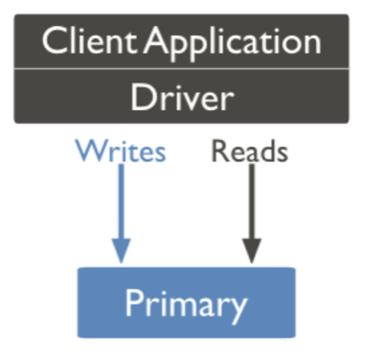
\includegraphics{1}
    \caption{Базовая структура кластера MongoDB}
    \label{fig:1}
\end{figure}

На рисунке~\ref{fig:2} показана типичная схема репликации MongoDB, в которой клиентскую программу всегда взаимодействует с первичным узлом, а первичный узел затем реплицирует данные на вторичные узлы.

\begin{figure}[H]
    \centering
    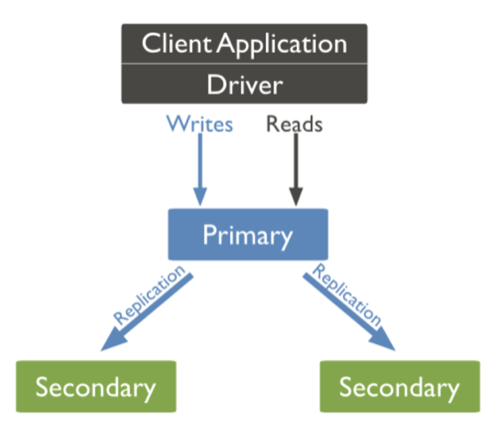
\includegraphics{2}
    \caption{Типичная схема репликации MongoDB}
    \label{fig:2}
\end{figure}

Особенности набора реплик:
\begin{itemize}
	\item кластер из N узлов;
	\item любой узел может быть основным;
	\item все операции записи идут на основной узел;
	\item автоматическое переключение при сбое;
	\item автоматическое обновление;
	\item консенсусные выборы первичного.
\end{itemize}

На рисунке~\ref{fig:3} изображена шардинг MongoDB с использованием сегментированного кластера.

\begin{figure}[H]
    \centering
    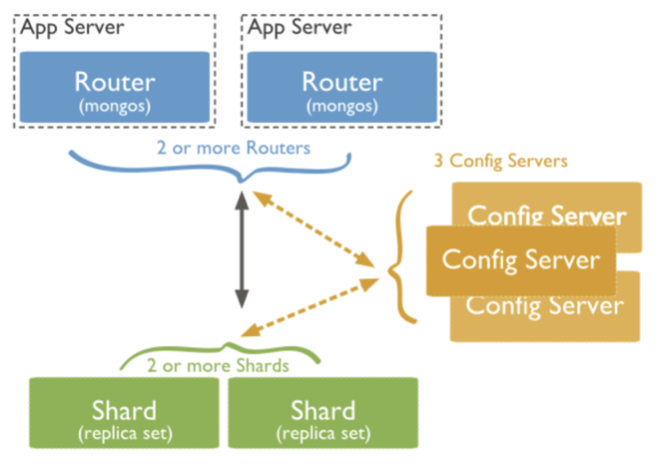
\includegraphics{3}
    \caption{Структура MongoDB при использовании шардинга}
    \label{fig:3}
\end{figure}

На данном рисунке есть три основных компонента:

Shards --- шарды, которые используются для хранения данных. Они обеспечивают высокую доступность и согласованность данных. В производственной среде каждый шард представляет собой отдельный набор реплик.

Config Servers --- серверы Config сохраняют метаданные кластера. Эти данные содержат сопоставление набора данных кластера с Шардена. Маршрутизатор запросов использует эти метаданные для нацеливания операций на определенные сегменты. В производственной среде сегментированные кластеры имеют ровно 3 сервера конфигурации.

Query Routers --- Query Routers --- это, в основном, экземпляры mongo, взамодействующие с клиентскими приложениями, направляя операции в соответствующий сегмент. Маршрутизатор обрабатывает и направляет операции на сегменты, а затем возвращает результаты клиентам. Кластерный кластер может содержать более одного маршрутизатора запросов для разделения нагрузки клиентских запросов. Клиент отправляет запросы одного маршрутизатора запросов. Как правило, в сегментированного кластера есть много маршрутизаторов запросов.

\subsection*{Выводы}
В рамках выполнения лабораторной работы были рассмотрены преимущества использования шардинга на серверах MongoDB и проведено развертывание сервера с использованием шардинга для улучшения показателей быстродействия обработки данных.

\end{document}
